\documentclass[answers]{exam}

\usepackage{amsmath}
\usepackage{amssymb}
\usepackage[spanish]{babel}
\usepackage{drawstack}
\usepackage{enumerate}
\usepackage[T1]{fontenc}
\usepackage{lmodern}
\usepackage{listings}
\usepackage{graphicx}
\usepackage{semantic}
\usepackage{stmaryrd}
\usepackage[cache=false,outputdir=./build]{minted}
\usepackage{xcolor} % to access the named colour LightGray
\definecolor{LightGray}{gray}{0.9}

% paquetes para escribir algoritmos y pseudocódigo
\usepackage{algpseudocode}
\usepackage{algorithm} 
\usepackage{algpseudocode} 
\renewcommand{\algorithmicrequire}{\textbf{Input:}} % Use Input in the format of Algorithm 
\renewcommand{\algorithmicensure}{\textbf{Output:}} % Use Output in the format of Algorithm
% paquetes para escribir algoritmos y pseudocódigo

\decimalpoint{}

\newcommand{\materia}{Programación Funcional}
\newcommand{\tarea}{Tarea 1}

\firstpageheadrule{}
\firstpageheader{
  Ramírez López Alvaro\\
  Numero de cuenta: 316276355
}{
  \materia{} \\
  \tarea{}
}{
  Fecha de entrega: \\
  24 de enero de 2023
}

\extrawidth{1.54cm}
\extraheadheight[5mm]{-5mm}
\renewcommand{\familydefault}{\sfdefault}

\renewcommand{\solutiontitle}{\noindent\textbf{Solución:}\par\noindent}
\runningheadrule{}
\runningheader{\materia{}}{\tarea{}}{\today}
\footer{}{Página \thepage\ de \numpages}{}

\lstset{basicstyle=\ttfamily,tabsize=3}
\definecolor{bg}{rgb}{0.95,0.95,0.95}

\begin{document}

\begin{questions}

\question{Indica la salida de cada una de las siguientes expresiones y verifica el resultado en \verb|DrRacket|.
\begin{itemize}
  \item \verb|(cons (+ 1 3) (cons (+ 5 6) (cons (- 3 2) empty)))|
  \item \verb|(list (+ 1 3) (+ 5 6) (- 3 2))|
  \item \verb|'((+ 1 3) (+ 5 6) (- 3 2))|
  \item \begin{verbatim}
(define a 0) 
(define xs '(10 20 30)) 
(cons a xs)
  \end{verbatim}
\end{itemize}
}

\begin{solution}
  \begin{itemize}
    \item \verb|(cons (+ 1 3) (cons (+ 5 6) (cons (- 3 2) empty)))|, la salida es: \verb|'(4 11 1)|
    \item \verb|(list (+ 1 3) (+ 5 6) (- 3 2))|, la salida es: \verb|'(4 11 1)|
    \item \verb|'((+ 1 3) (+ 5 6) (- 3 2))|, la salida es: \verb|'((+ 1 3) (+ 5 6) (- 3 2))|
    \item \begin{verbatim}
(define a 0) 
(define xs '(10 20 30)) 
(cons a xs)
    \end{verbatim}
    la salida es: \verb|'(0 10 20 30)|
  \end{itemize}

  La comprobacion aqui esta:
    %% insertar imagen
    \begin{center}
      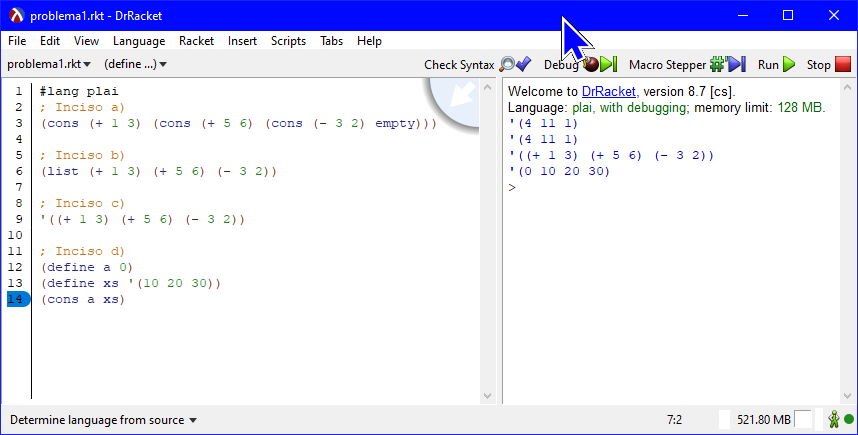
\includegraphics[scale=.65]{images/1.png}
    \end{center}
\end{solution}

\question{Realiza los siguientes ejercicios en el orden indicado. El objetivo de este ejercicio es aprender a usar la
documentacion de Racket. En este caso, debes consultar la documentacion de Pares y Lista.
\begin{enumerate}
  \item Construye una lista con el nombre de tus canciones favoritas (de preferencia mas de 5) usando cons o list, el que mas te guste. Dale un nombre con define.
  \item Investiga como verificar si una lista esta vacía, anota el nombre de la función y úsala para verificar que en efecto tu lista no esta vacía.
  \item Investiga como obtener el numero de elementos de una lista, anota el nombre de la función y úsala para conocer el numero de elementos de tu lista.
  \item Investiga como obtener el primer elemento de una lista, anota el nombre de la función y úsala con tu lista.
  \item Crea otra lista, ahora con el nombre de tus películas favoritas (igual mas de 5). Dale un nombre con define. Debe ser distinta de la primera.
  \item Investiga como concatenar dos listas, anota el nombre de la función y úsala para crear una nueva lista que sea la concatenación de las dos anteriores. Dale un nombre con define. Debe ser distinto a la primera y a la segunda.
  \item Investiga como eliminar un elemento de una lista (a partir de un indice), anota su nombre y úsala para quitar el segundo elemento de la primera lista, el tercero de la segunda y el cuarto de la tercera.
\end{enumerate}
}

\begin{solution}
  \begin{enumerate}
    \item Para el este inciso, la respuesta se vería asi: 
    \begin{verbatim}
(define miMusica (list "Information High" "Sin Frenos" "Tu y yo" "Asi soy" "Muchacha"))
    \end{verbatim}
    \item Para el este inciso, la respuesta se vería asi: \verb|(empty? miMusica)|
    \item Para el este inciso, la respuesta se vería asi: \verb|(length miMusica)|
    \item Para el este inciso, la respuesta se vería asi: \verb|(car miMusica)|
    \item Para el este inciso, la respuesta se vería asi: 
    \begin{verbatim}
(define misPeliculas 
  (cons "Commando" 
    (cons "El demoledor" 
      (cons "Terminator" 
        (cons "Cobra" 
          (cons "Volver al futuro" empty))))))
    \end{verbatim} 
    \item Para el este inciso, la respuesta se vería asi: \verb|(define dosListas (append miMusica misPeliculas))|
    \item Para el este inciso, la respuesta se vería asi:
    \begin{verbatim}
(define (removeIndex i lista)
  (append (take lista (- i 1)) (drop lista i)))

(removeIndex 2 miMusica)
(removeIndex 3 misPeliculas)
(removeIndex 4 dosListas)
    \end{verbatim}
  \end{enumerate}
  Aqui esta la comprobacion en DrRacket
% insertar imagen
  \begin{center}
    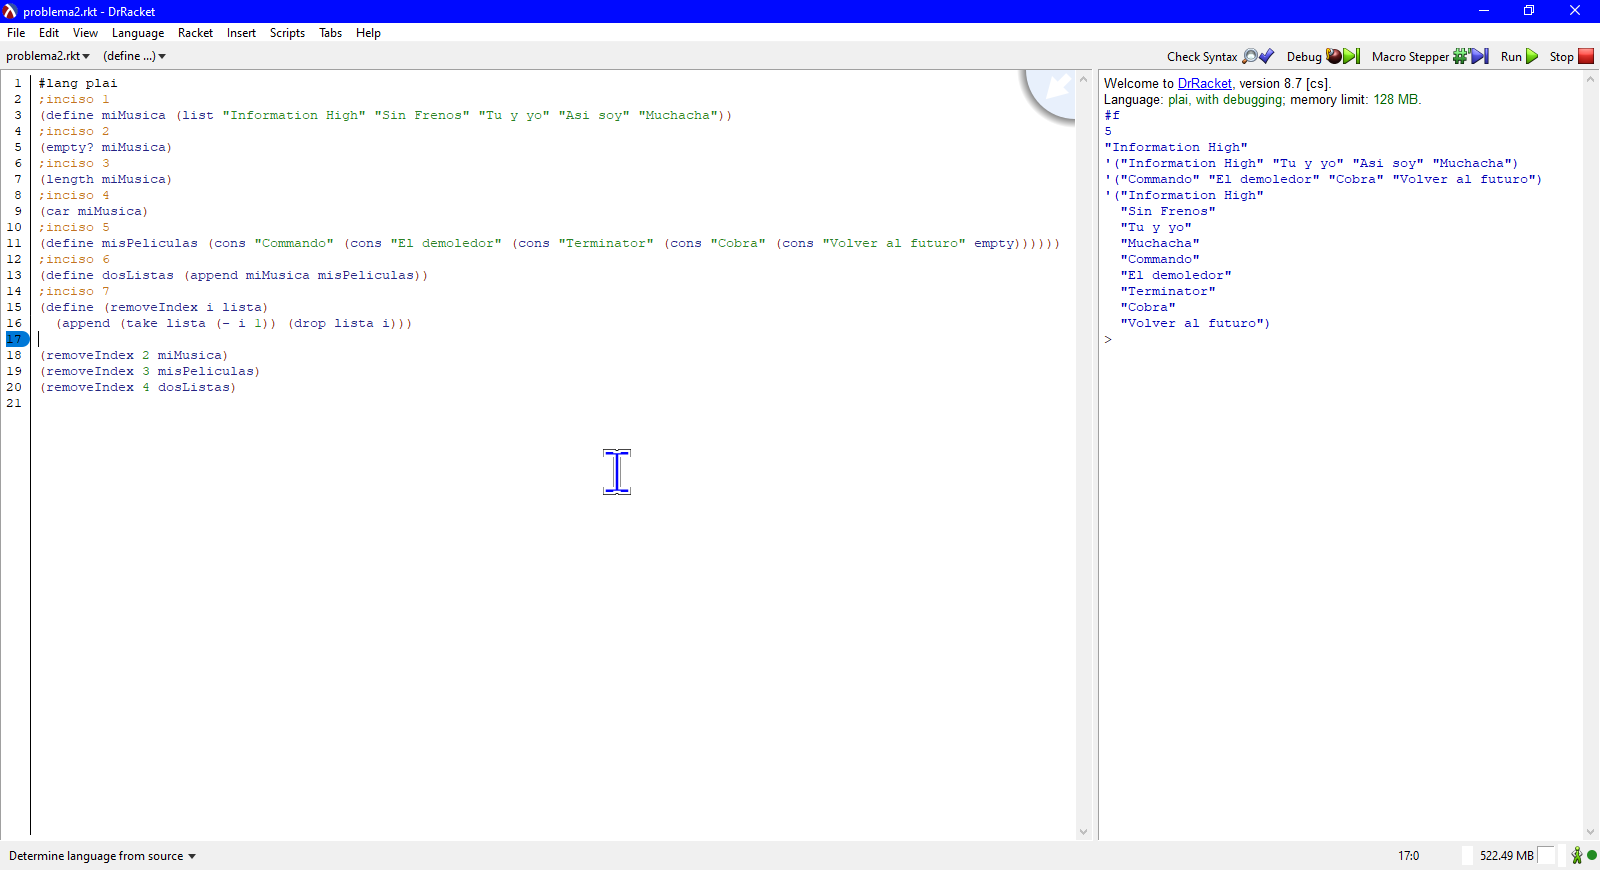
\includegraphics[scale=.4]{images/2.png}
  \end{center}

\end{solution}
\end{questions}

\end{document}